\section{Performance Impact of Load Balancer Scale}
% 1 page
With this experiment we evaluate the effect different load balancer scales have on the system.
As we already described the quality and thus resulting end user performance of load balancer decisions only stabilizes after a while, since the load balancer first has to evaluate the available upstreams by sending requests to them.
Because of this, having larger numbers of load balancers present in the system might lead to delayed convergence, and thus suboptimal performance.
Having too few load balancers, on the other hand, might lead to lost performance through overly long routes.

To find out how different scales affect the overall system, we test the system performance with fixed percentages of nodes hosting load balancers.
We test a ranges between 5\% and 100\% of nodes hosting load balancers, which in our scenarios across three cities and 400 nodes means between 20 and 400 load balancer instances.
Scheduling load balancer replicas in these scenarios is still left to the Kubernetes scheduler, which means that the location of the node in the topology is not taken into account.

When testing ratios where less than 5\% of nodes hosted load balancers, we ran into frequent occurrences of the simulation not terminating within a feasible time window.
Upon investigation it turned out that if a load balancer was the only one in the city, or otherwise handled a lot of traffic, but happened to be placed onto a node with very limited bandwidth, the network simulation would take an exceedingly long time.
Requests that did go through took so long, that in real-life it would be considered a failed request by timeout.
We take this as an indication of the inherent problematic of current replica scheduling methods in edge computing, and that the usage of current techniques would simply require an outsized number of load balancers to mitigate the risk of such dysfunctional configurations.

The topologies tested are structurally similar to those of the initial evaluation.
Our two testing scenarios are three cities distributed across the United States, and three cities distributed across the globe.
The cities are identical to the ones from the initial evaluation, and feature identical network latencies between them.
The difference between these and the ones of the initial evaluation is that these feature a different internal topology, which is more closely related to edge intelligence\cite{rauschEdgeIntelligenceConvergence2019} and edge computing in general.
The cities in this evaluation have their compute capabilities, i.e. the cluster nodes, either in the city's local cloud data center, on a smart pole, or next to a cellular base station.
Clients are attached either to smart poles or directly to cellular base stations.
Cellular base stations themselves have a high-speed, high-bandwidth uplink to the wider network and feature a lower bandwidth and higher latency wireless connection to the clients.
These wireless properties depend on whether the cellular tower is LTE or 5G based, as both types are present in our scenario and their network properties are based on real world data\cite{braudMulticarrierMeasurementStudy2019}.
Not all cellular towers have directly attached compute capabilities.
In addition, one of the three cities does not feature a data center.

We simulate the cluster over the course of 2000 seconds, once with 25 \gls{rps}, once with 75\gls{rps}.

\begin{table}[]
\begin{tabular}{lrrrr}
\hline
                                                                             & \multicolumn{4}{c}{mean}                                                                                                                                                                                                                                              \\
\textbf{\begin{tabular}[c]{@{}l@{}}Nodes with\\ Load Balancers\end{tabular}} & \textbf{\begin{tabular}[c]{@{}r@{}}Global\\ 75rps\end{tabular}} & \textbf{\begin{tabular}[c]{@{}r@{}}Global\\ 25rps\end{tabular}} & \textbf{\begin{tabular}[c]{@{}r@{}}Nation\\ 75rps\end{tabular}} & \textbf{\begin{tabular}[c]{@{}r@{}}Nation\\ 25rps\end{tabular}} \\ \hline
\textbf{5\%}                                                                 & 210ms                                                           & 132ms                                                           & 220ms                                                           & 141ms                                                           \\
\textbf{10\%}                                                                & 149ms                                                           & 128ms                                                           & 158ms                                                           & 133ms                                                           \\
\textbf{20\%}                                                                & 134ms                                                           & 127ms                                                           & 147ms                                                           & 128ms                                                           \\
\textbf{30\%}                                                                & 132ms                                                           & 124ms                                                           & 141ms                                                           & 127ms                                                           \\
\textbf{40\%}                                                                & 130ms                                                           & 126ms                                                           & 135ms                                                           & 126ms                                                           \\
\textbf{50\%}                                                                & 128ms                                                           & 125ms                                                           & 134ms                                                           & 125ms                                                           \\
\textbf{60\%}                                                                & 129ms                                                           & 126ms                                                           & 133ms                                                           & 126ms                                                           \\
\textbf{70\%}                                                                & 129ms                                                           & 125ms                                                           & 128ms                                                           & 126ms                                                           \\
\textbf{80\%}                                                                & 128ms                                                           & 128ms                                                           & 131ms                                                           & 125ms                                                           \\
\textbf{90\%}                                                                & 129ms                                                           & 125ms                                                           & 129ms                                                           & 125ms                                                           \\
\textbf{100\%}                                                               & 127ms                                                           & 125ms                                                           & 129ms                                                           & 126ms                                                           \\ \hline
\end{tabular}
\caption{Mean \gls{trt} values of different load balancer scales, once they have converged to a stable value}
\label{tab:lb_scaling_converged_trt}
\end{table}

\begin{figure}
    \centering
    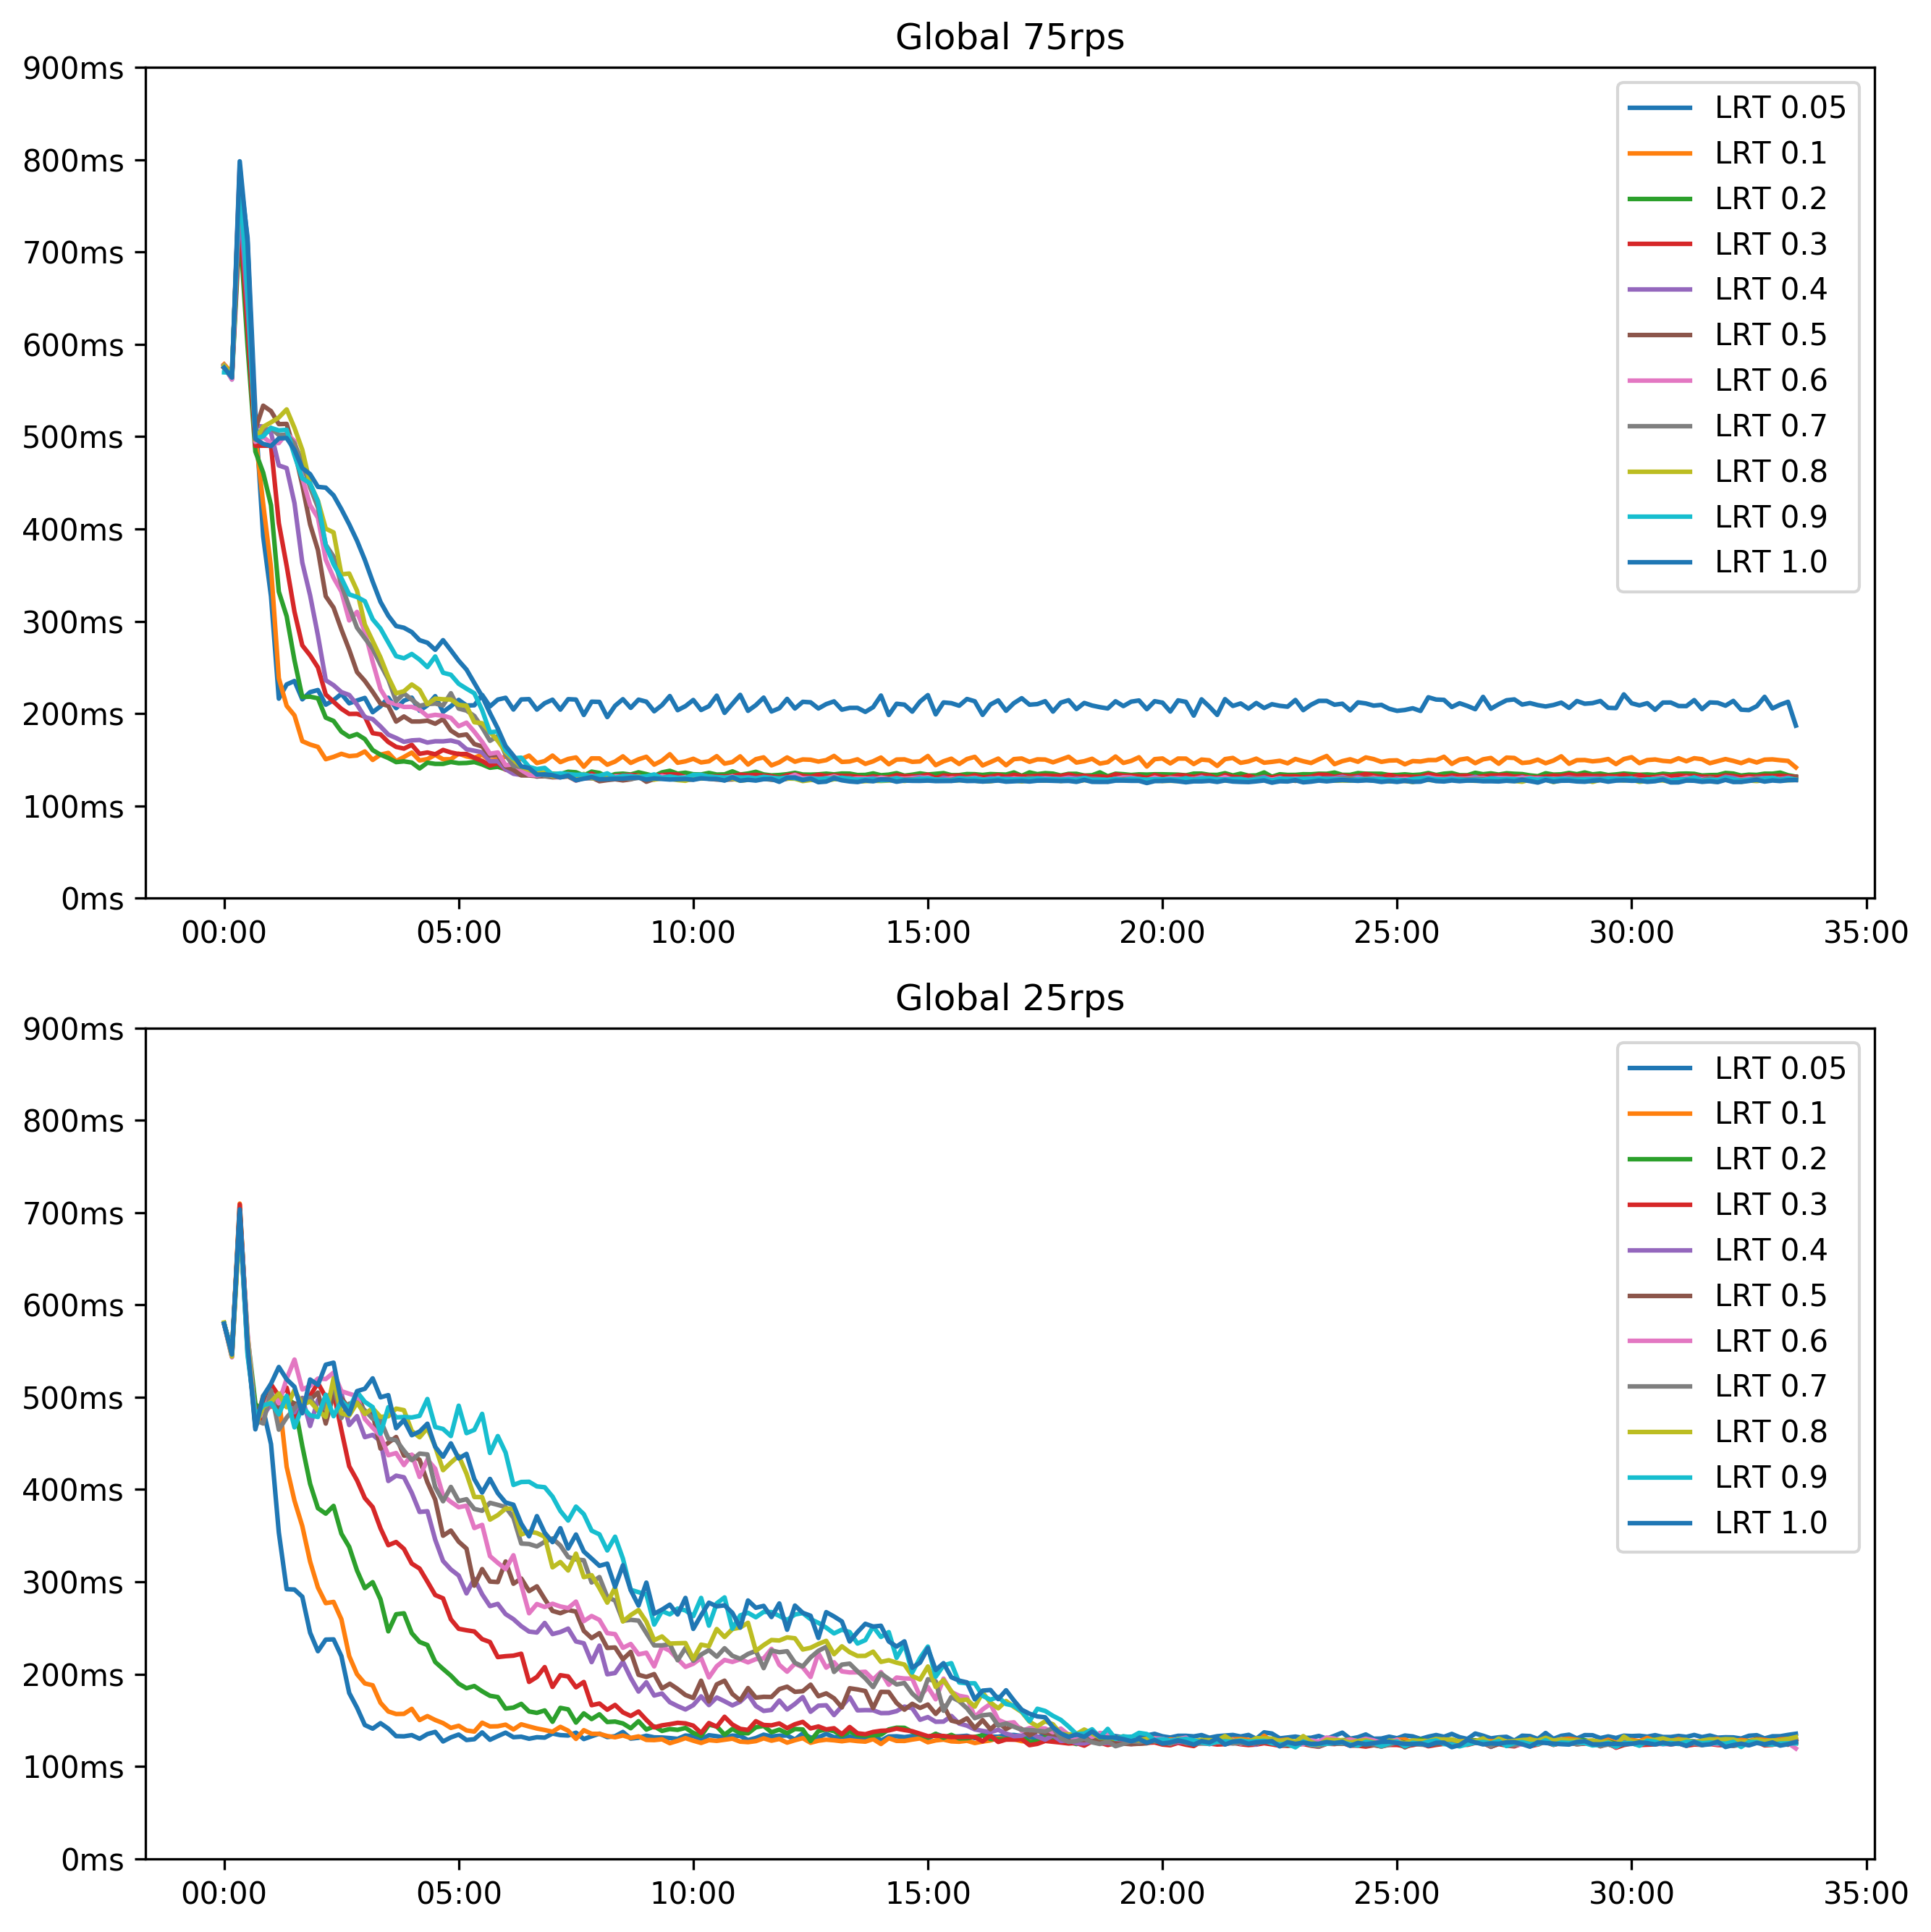
\includegraphics[width=\linewidth]{graphics/graphs/global_lb_scale.png}
    \caption{\glspl{trt} of different load balancer scales in the global scenario. For legibility a 10 second moving average is applied.}
    \label{fig:lb_scale_global}
\end{figure}

\begin{figure}
    \centering
    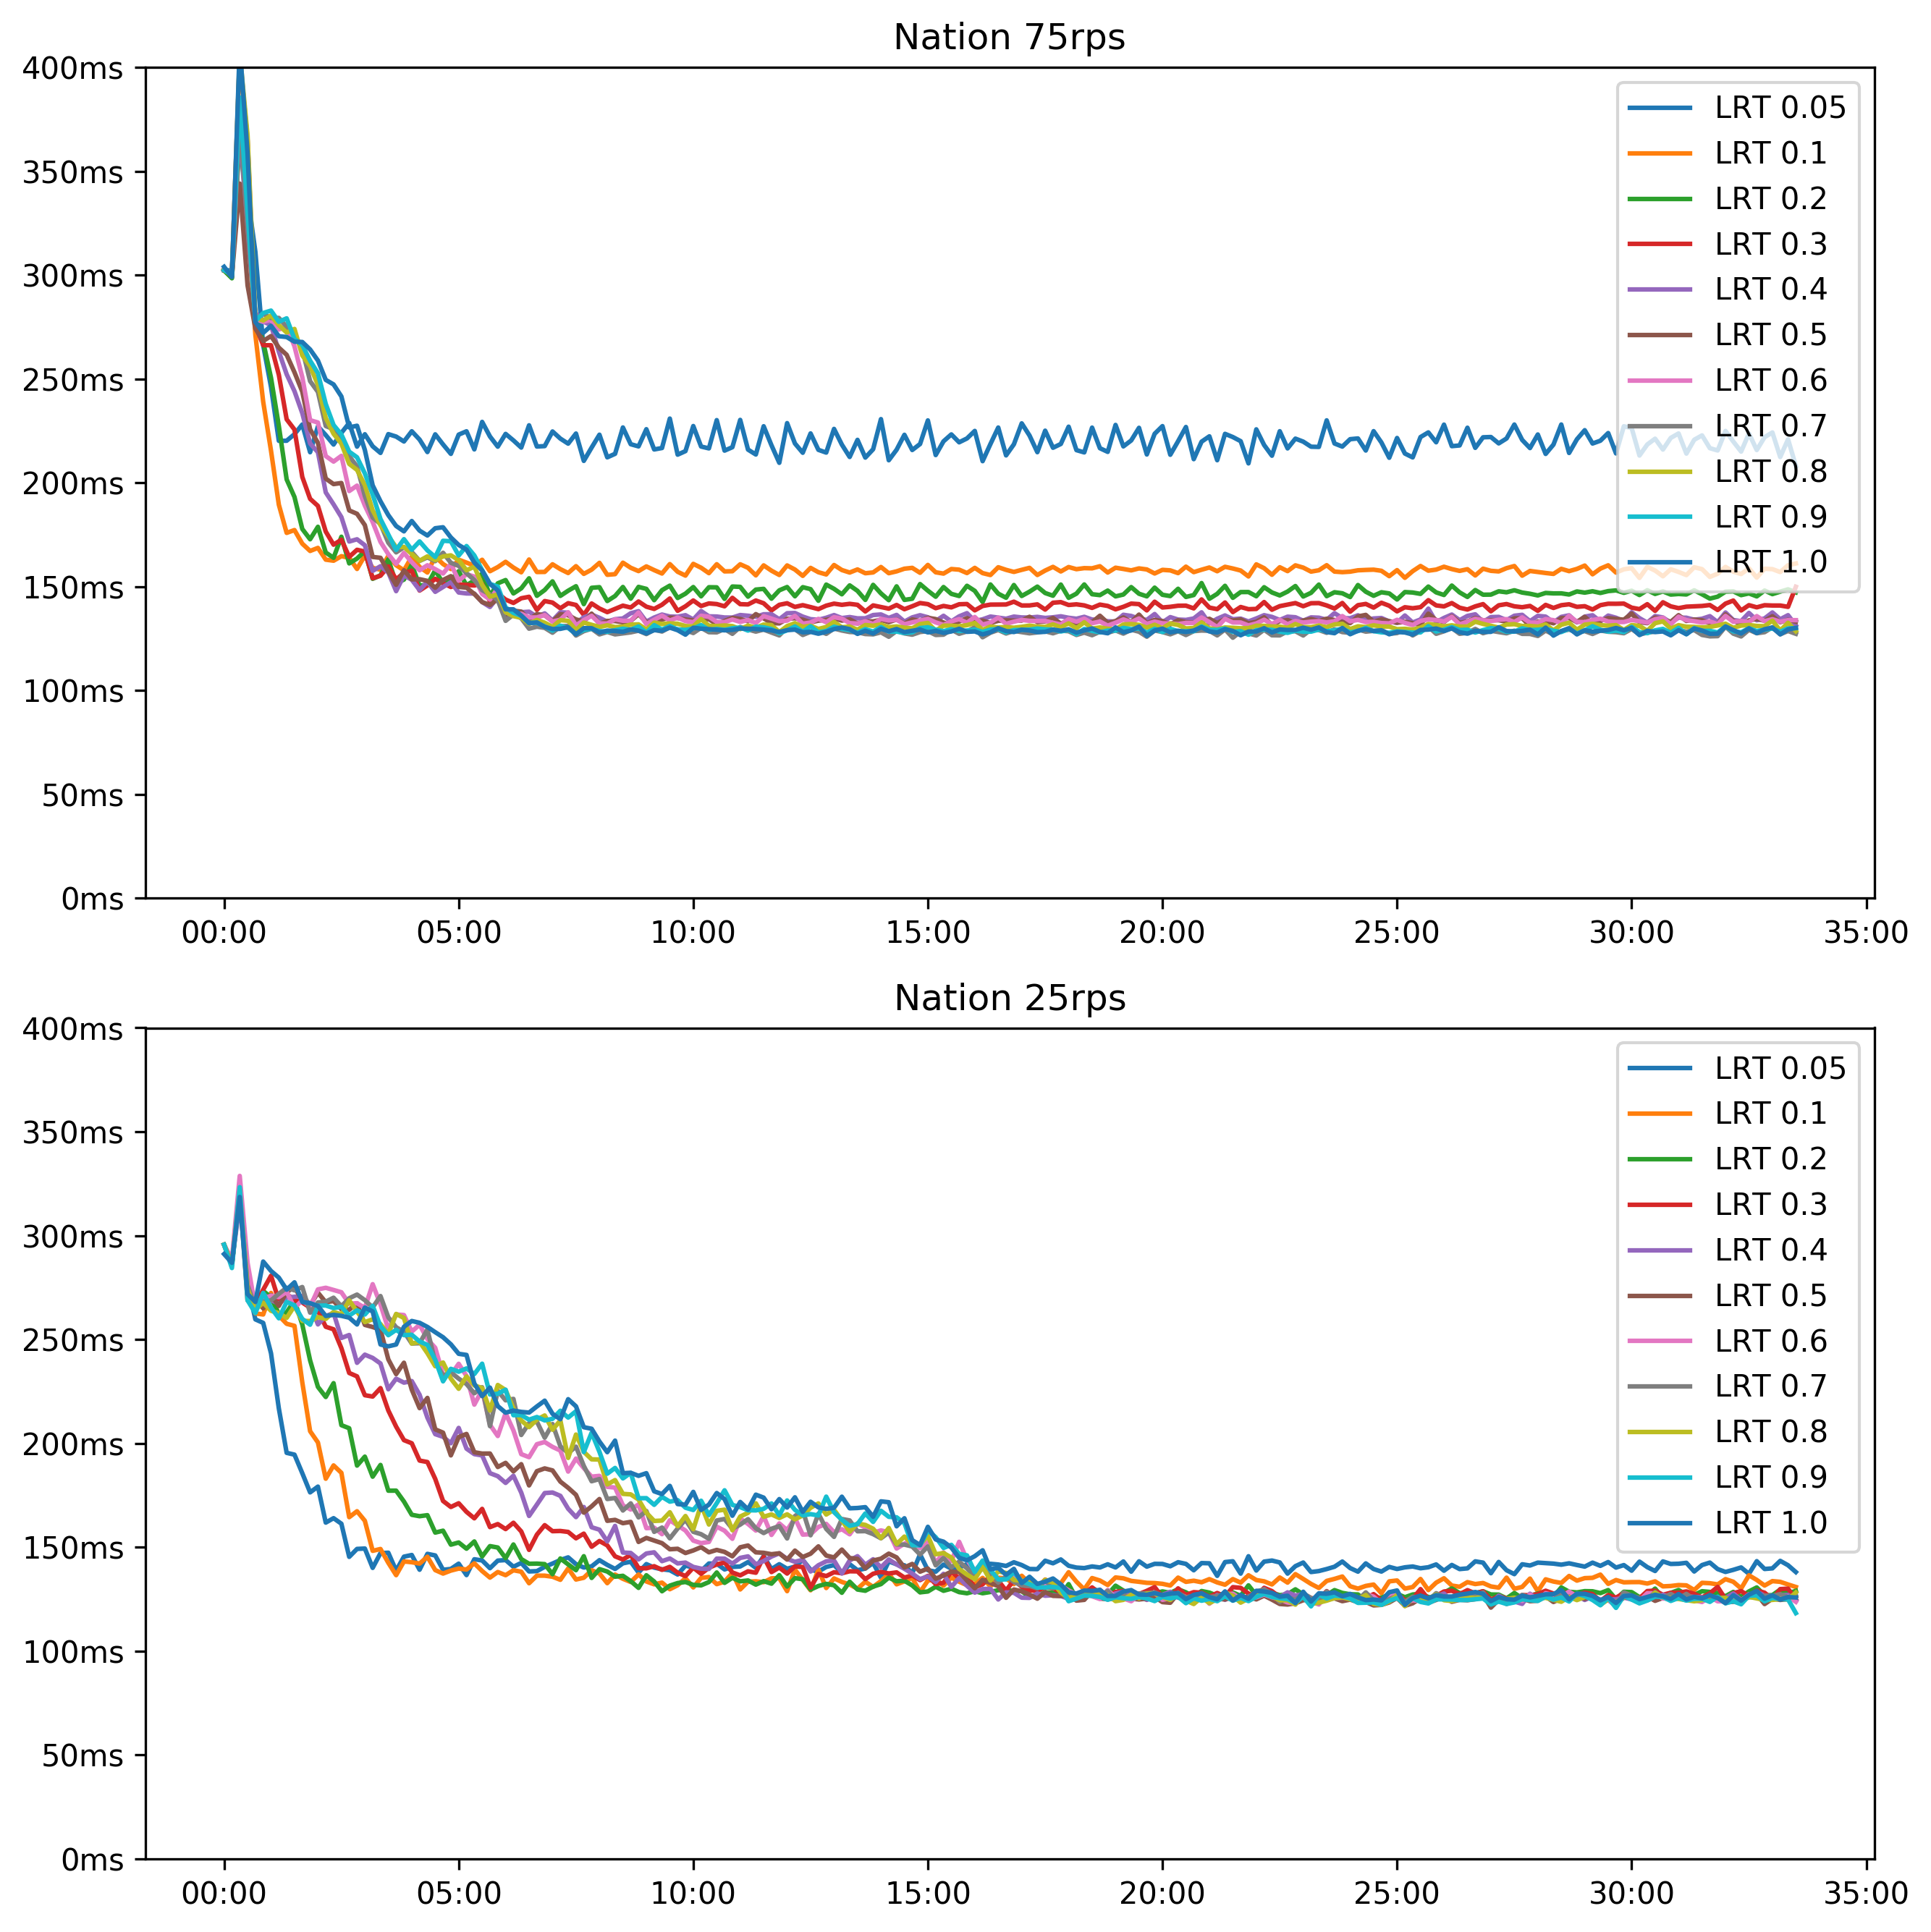
\includegraphics[width=\linewidth]{graphics/graphs/nation_lb_scale.png}
    \caption{\glspl{trt} of different load balancer scales in the nation scenario. For legibility a 10 second moving average is applied.}
    \label{fig:lb_scale_nation}
\end{figure}

Our results show consistent patterns across both topologies, but differ across the request rate.
While in scenarios with a request rate of 75 \gls{rps} higher numbers of load balancers lead to improved mean response time, in scenarios with 25 \gls{rps} lower numbers perform better.
Figures \ref{fig:lb_scale_global} and \ref{fig:lb_scale_nation} show explanations for this behaviour.
With lower numbers of load balancers the request rate per load balancer is higher, and thus leads to faster convergence towards a stable and efficient response time.

Table \ref{tab:lb_scaling_converged_trt} shows the mean response times of different load balancer scales once response times have stabilized.
Once only stabilized values are considered higher numbers of load balancers lead to improved performance.
Figures \ref{fig:lb_scale_global} and \ref{fig:lb_scale_nation} show this too, where lower numbers of load balancers stabilize earlier, but at higher \gls{trt} values.
From Table \ref{tab:lb_scaling_converged_trt} we also see that between the different load balancer scales, differences in response time become negligible at a certain point, with load balancers on 50\% of nodes converging to almost the same mean response time as having load balancers on 100\% of nodes.

Lastly, we observe that the absolute difference between the time when the system performs best, and when the system performs worst is dependent on topology make up.
The globally distributed scenario has the potential to perform worse, as there is a greater likelihood of poor request routing decisions resulting in longer network distances.
